\documentclass{article}

% if you need to pass options to natbib, use, e.g.:
%     \PassOptionsToPackage{numbers, compress}{natbib}
% before loading neurips_2020

% ready for submission
% \usepackage{neurips_2020}

% to compile a preprint version, e.g., for submission to arXiv, add add the
% [preprint] option:
%     \usepackage[preprint]{neurips_2020}

% to compile a camera-ready version, add the [final] option, e.g.:
%     \usepackage[final]{neurips_2020}

% to avoid loading the natbib package, add option nonatbib:
     \usepackage[nonatbib]{neurips_2020}

\usepackage[utf8]{inputenc} % allow utf-8 input
\usepackage[T1]{fontenc}    % use 8-bit T1 fonts
\usepackage{hyperref}       % hyperlinks
\usepackage{url}            % simple URL typesetting
\usepackage{booktabs}       % professional-quality tables
\usepackage{amsfonts}       % blackboard math symbols
\usepackage{nicefrac}       % compact symbols for 1/2, etc.
\usepackage{microtype}      % microtypography
\usepackage{chemformula}

\title{Deep Reinforcement Learning to Minimize Long-Term Carbon Emissions and Cost in Electricity Generation Investment}

% The \author macro works with any number of authors. There are two commands
% used to separate the names and addresses of multiple authors: \And and \AND.
%
% Using \And between authors leaves it to LaTeX to determine where to break the
% lines. Using \AND forces a line break at that point. So, if LaTeX puts 3 of 4
% authors names on the first line, and the last on the second line, try using
% \AND instead of \And before the third author name.

\author{%
  David S.~Hippocampus\thanks{Use footnote for providing further information
    about author (webpage, alternative address)---\emph{not} for acknowledging
    funding agencies.} \\
  Department of Computer Science\\
  Cranberry-Lemon University\\
  Pittsburgh, PA 15213 \\
  \texttt{hippo@cs.cranberry-lemon.edu} \\
  % examples of more authors
  % \And
  % Coauthor \\
  % Affiliation \\
  % Address \\
  % \texttt{email} \\
  % \AND
  % Coauthor \\
  % Affiliation \\
  % Address \\
  % \texttt{email} \\
  % \And
  % Coauthor \\
  % Affiliation \\
  % Address \\
  % \texttt{email} \\
  % \And
  % Coauthor \\
  % Affiliation \\
  % Address \\
  % \texttt{email} \\
}

\begin{document}

\maketitle

\begin{abstract}

{\color{red}Placeholder}: A transition from a high carbon electricity supply to a low-carbon system is central to avoiding catastrophic climate change \cite{Kell2020}. Much of the work in decarbonisation relies on a low-carbon electricity supply, such as cooling, heating and automotive, amongst others. Such a transition must be made in a gradual approach to avoid frequent collapse of the electricity supply.

Renewable energy costs, such as solar and wind sources, have dropped in price making them cost competitive with fossil fuels. This is projected to continue into the future \cite{IEA2015}. The future cost of generation, demand and fuel prices, however, remain uncertain over the long-term future. These uncertainties are risks which investors must analyse while making long-term investment decisions.

\end{abstract}




\section{Introduction}
\label{sec:intro}


A transition from a high carbon electricity supply to a low-carbon system is central to avoiding catastrophic climate change \cite{Kell2020}. Much of the work in decarbonisation relies on a low-carbon electricity supply, such as cooling, heating and automotive, amongst others. Such a transition must be made in a gradual approach to avoid frequent collapse of the electricity supply.

Renewable energy costs, such as solar and wind sources, have dropped in price making them cost competitive with fossil fuels. This is projected to continue into the future \cite{IEA2015}. The future cost of generation, demand and fuel prices, however, remain uncertain over the long-term future. These uncertainties are risks which investors must analyse while making long-term investment decisions.

In this paper, we use the deep deterministic policy gradient (DDPG) reinforcement learning algorithm to simulate the behaviour of investors over a 50-year horizon \cite{Hunt2016a}. The environment used was a modified version of the FTT:Power model \cite{Mercure2012}. FTT:Power is a global power systems model that uses logistic differential equations to simulate technology switching. 

We modified the FTT:Power model to use the DDPG algorithm in place of the logistic differential equations to simulate investment decisions, as well as only simulating two countries: the United Kingdom and Ireland. The DDPG algorithm allowed us to simulate the decisions made by investors made under imperfect information over a 50-year period. That is, they did not have knowledge of future demand, fuel and generation costs. 

The reinforcement learning algorithm enabled us to model the behaviour of an investor without perfect knowledge of the future, with a view to reduce carbon emissions and overall cost of the system. The reinforcement learning agent is a single actor that invests in both the UK and Ireland. This work enabled us to see whether a low-carbon mix is possible over the next 50-years to avert climate change.

Through this work, it is possible to assess whether a low cost, low-carbon electricity mix is viable over the long-term using a deep reinforcement learning investment algorithm. Our approach is in contrast to a mixed-integer linear programming problem, where full knowledge of the time-horizon is required.

Oliveira \textit{et al.} also use reinforcement learning for the capacity expansion problem~\cite{Oliveira2018}. They, however, focus on a 20-year time horizon. Kazempour \textit{et al.} use a mixed integer linear programming approach to solve the generation investment problem \cite{Kazempour2011}. In this work, we address a gap in the literature for the capacity expansion problem over a 60 year time period using deep reinforcement learning to reduce both carbon emissions and electricity price.




%\begin{itemize}
%	\item Requirement to reduce carbon emissions globally.
%	\item This must be achieved cost effectively.
%	\item Requirement for a global solution to find optimal mix of electricity mix with imperfect information about the future (eg. costs and demand).
%	\item Use of reinforcement learning to take into account all uncertainties to achieve goal of a cost effective and low-carbon solution
%	\item Use of FTT:Power model to simulate investment in the UK and Ireland over a 50 year horizon
%	\item Examples of existing literature
%\end{itemize}


\section{Model and methodology}
\label{sec:methods}


In this paper, we used the Future Technology Transformations for the power sector  model (FTT:Power). This model represents global power systems based on market competition, induced technological change and natural resource use and depletion. Induced technological change occurs through technological learning produced by cumulative investment and leads to nonlinear path dependent technological transitions \cite{Mercure2012}. The model uses a dynamic set of logistic differential equations for competition between technology options.

For this work, however, we modified the FTT:Power model to use the deep reinforcement learning investment algorithm, DDPG. That is, the size of the investment made in each technology was made by the DDPG algorithm. In addition, we reduced the model to only consider the countries of Ireland and the UK. This enabled us to iterate through enough episodes for the reinforcement learning to converge to an optimal reward.

\subsection*{Reinforcement Learning}

The investment decision making process can be formulated as a Markov Decision Process (MDP) \cite{puterman2014markov}. In an MDP environment, an agent receives an observation about the state of their environment $s_t$, chooses an action $a_t$ and receives a reward $r_t$ based upon their environment and action. Solving an MDP consists of maximising the cumulative reward over the lifetime of the agent. 


For our simulation environment, the agent makes a continuous investment decision for each energy technology, in each region and each year, starting from 2017 until 2060. 	Technology switching is modelled using a pairwise comparison of flows of market shares of different electricity generation capacity. That is, how much capacity flows from one technology to another. 

The agent's observation space is a matrix consisting of the electricity produced by each technology, total capacity, total \ch{CO2} emissions over the simulation, levelized cost of electricity (LCOE) both including taxes and not including taxes, cumulative investment in each technology, investment in new capacity, carrier prices by commodity, fuel costs and carbon costs.

The reward $r$ is defined as:
\begin{equation}
	r = -\left(1000\times\ch{CO2}_e + \frac{LCOE}{1000}\right),
\end{equation}

where $\ch{CO2}_e$ is equal to total \ch{CO2} emissions over the simulation, and $LCOE$ is equal to LCOE, excluding taxes. The scaling factors were used to place the $LCOE$ and $\ch{CO2}$ on the same scale. The reward was multiplied by -1 due to the RL algorithm maximising reward and our requirement to reduce both LCOE and \ch{CO2} emissions.


RL approaches have been used to solve MDP \cite{Sutton2015}. In recent times, however, RL has been extended to incorporate Deep Reinforcement Learning (DRL). DRL relies on deep neural networks to overcome the problems of memory complexity and computation complexity \cite{Arulkumaran2017}. 

We applied the deep deterministic policy gradient (DDPG) DRL algorithm \cite{Hunt2016a} from the Ray RLlib package \cite{Liang2014}. The DDPG algorithm is made up of an actor and critic network. We designed both of these to have two hidden layers, made up of 400 and 300 units per layer. The training batch size was set to 40,000. We chose these numbers due to their implementation in Ray RLlib and our inability to tune the hyper-parameters, due to a two week running time.

% Sample batch size = 10000
% Train batch size = 40000

% EndYear = 2050
% N = 149

% observations = [G_cum, U_cum, E_cum, CF_cum, LCOE_cum, TLCOE_cum, W_cum, I_cum, P_cum, Fcosts_cum, CO2_costs_cum];

% Electricity produced by technology
% Total capacity
% Emissions of CO2 during year
% Capacity factor
% LCOE excluding taxes and carbon price
% Levelised cost including taxes
% Cumulative investment (global)
% Investment in new capacity
% P_cum: Carrier prices by commodity
% Fcosts_cum: Fuel costs
% C02_costs_cum: Carbon costs

%
%\begin{itemize}
%	\item Use of simplified FTT:Power model (Ireland + UK)
%	\item Explain DDPG algorithm
%	\item Detail how we adopted the algorithm to minimize both cost and carbon emissions
%\end{itemize}



\section{Results}
\label{sec:results}


%\begin{figure*}
%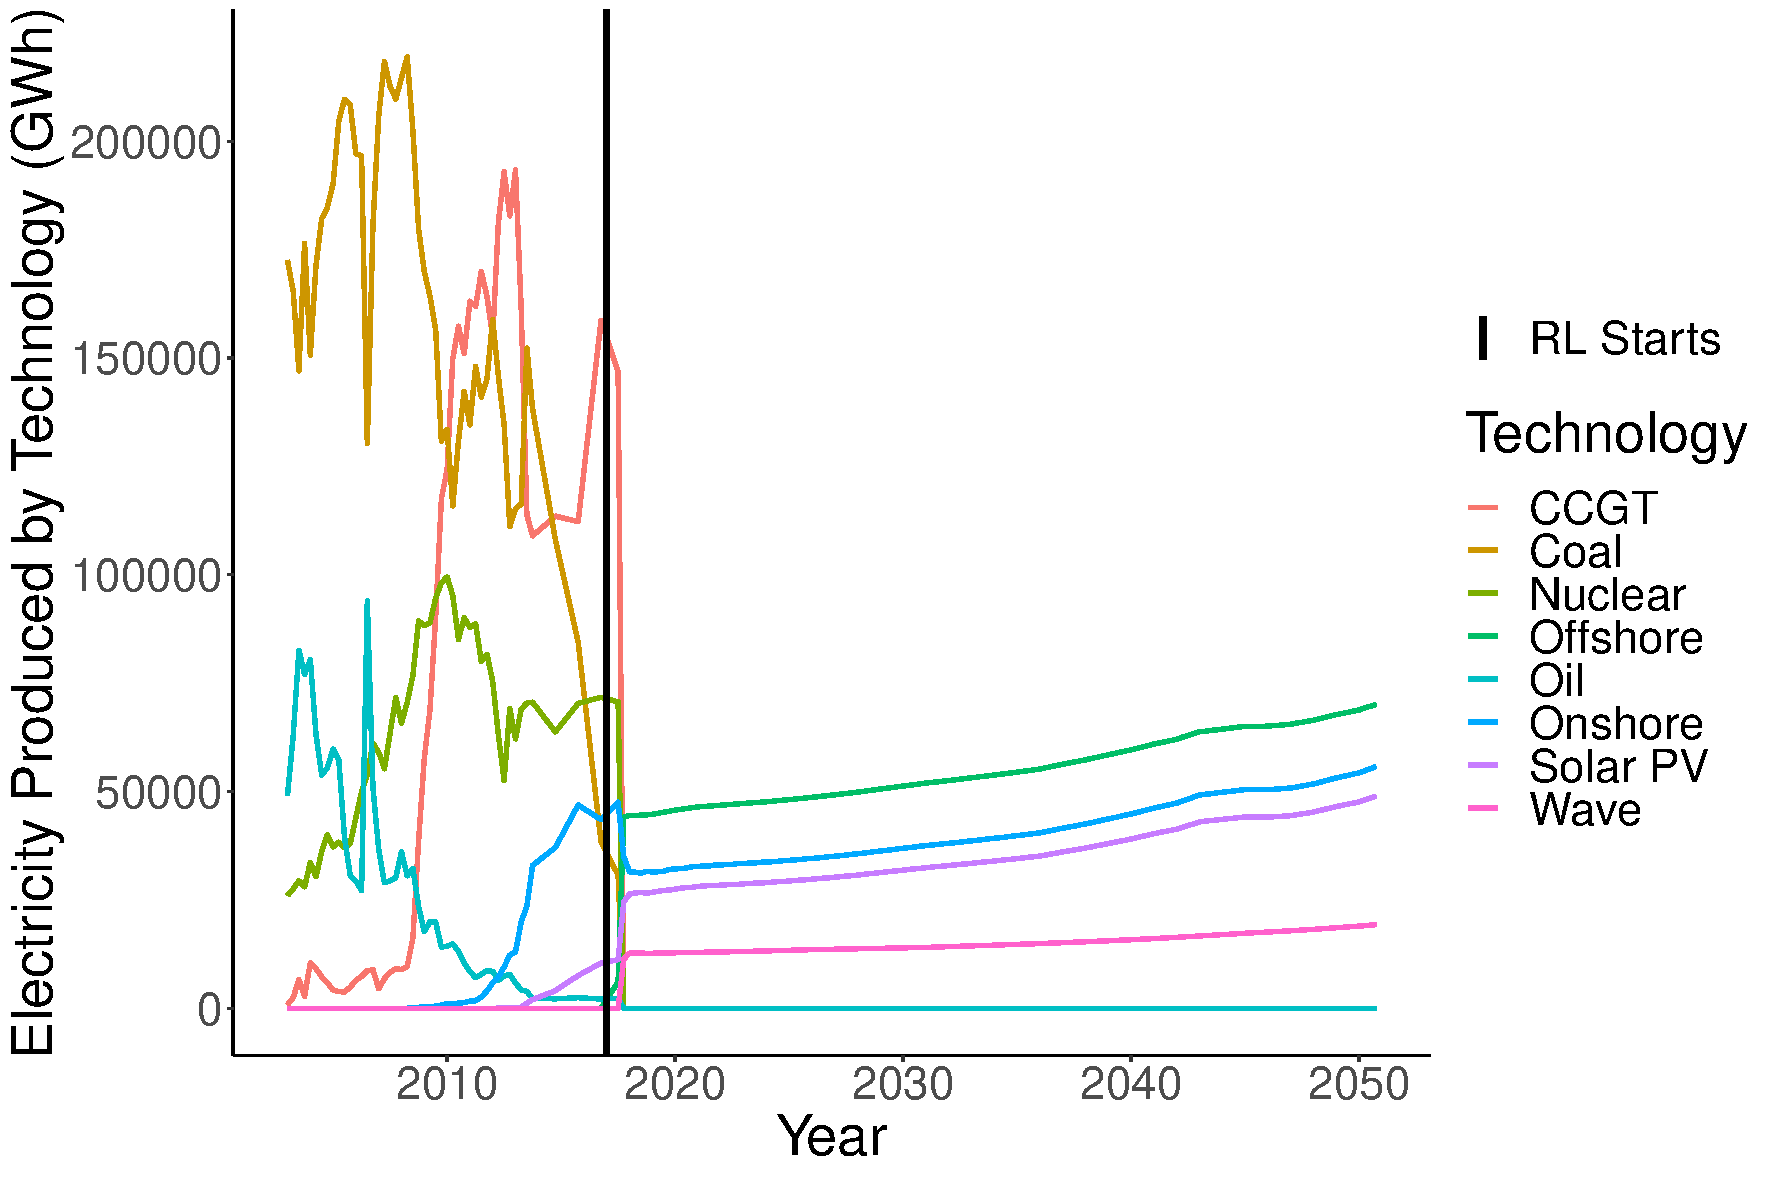
\includegraphics[width=0.8\columnwidth]{figures/electricity_generated_plot.pdf}
%\label{fig:electricity_generated_plot}
%\caption{Mean outputs of various technologies vs. mean absolute error from 2018 to 2035 in ElecSim.}
%\end{figure*}
%
%\begin{figure*}
%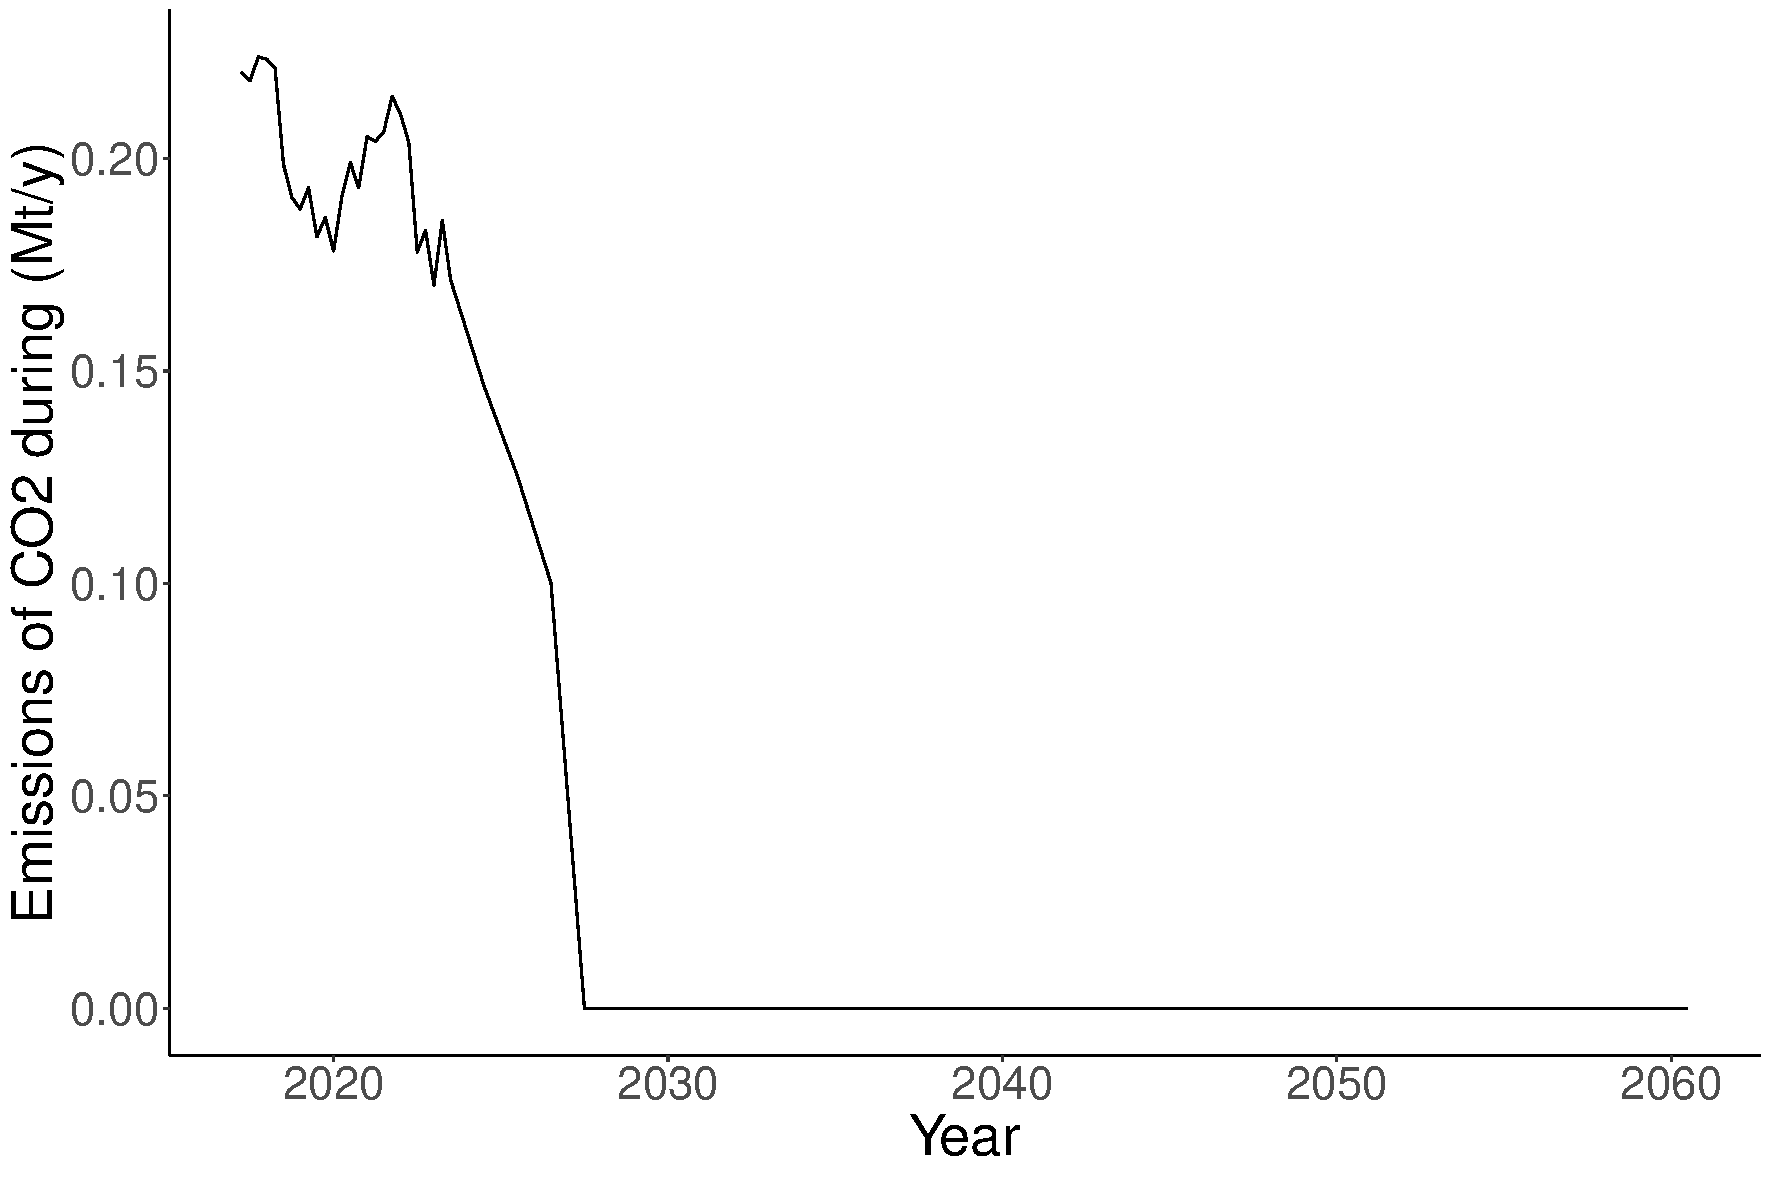
\includegraphics[width=0.8\columnwidth]{figures/emissions_plot.pdf}
%\label{fig:electricity_generated_plot}
%\caption{Mean outputs of various technologies vs. mean absolute error from 2018 to 2035 in ElecSim.}
%\end{figure*}

\begin{figure}
\centering
\begin{minipage}{.5\textwidth}
  \centering
  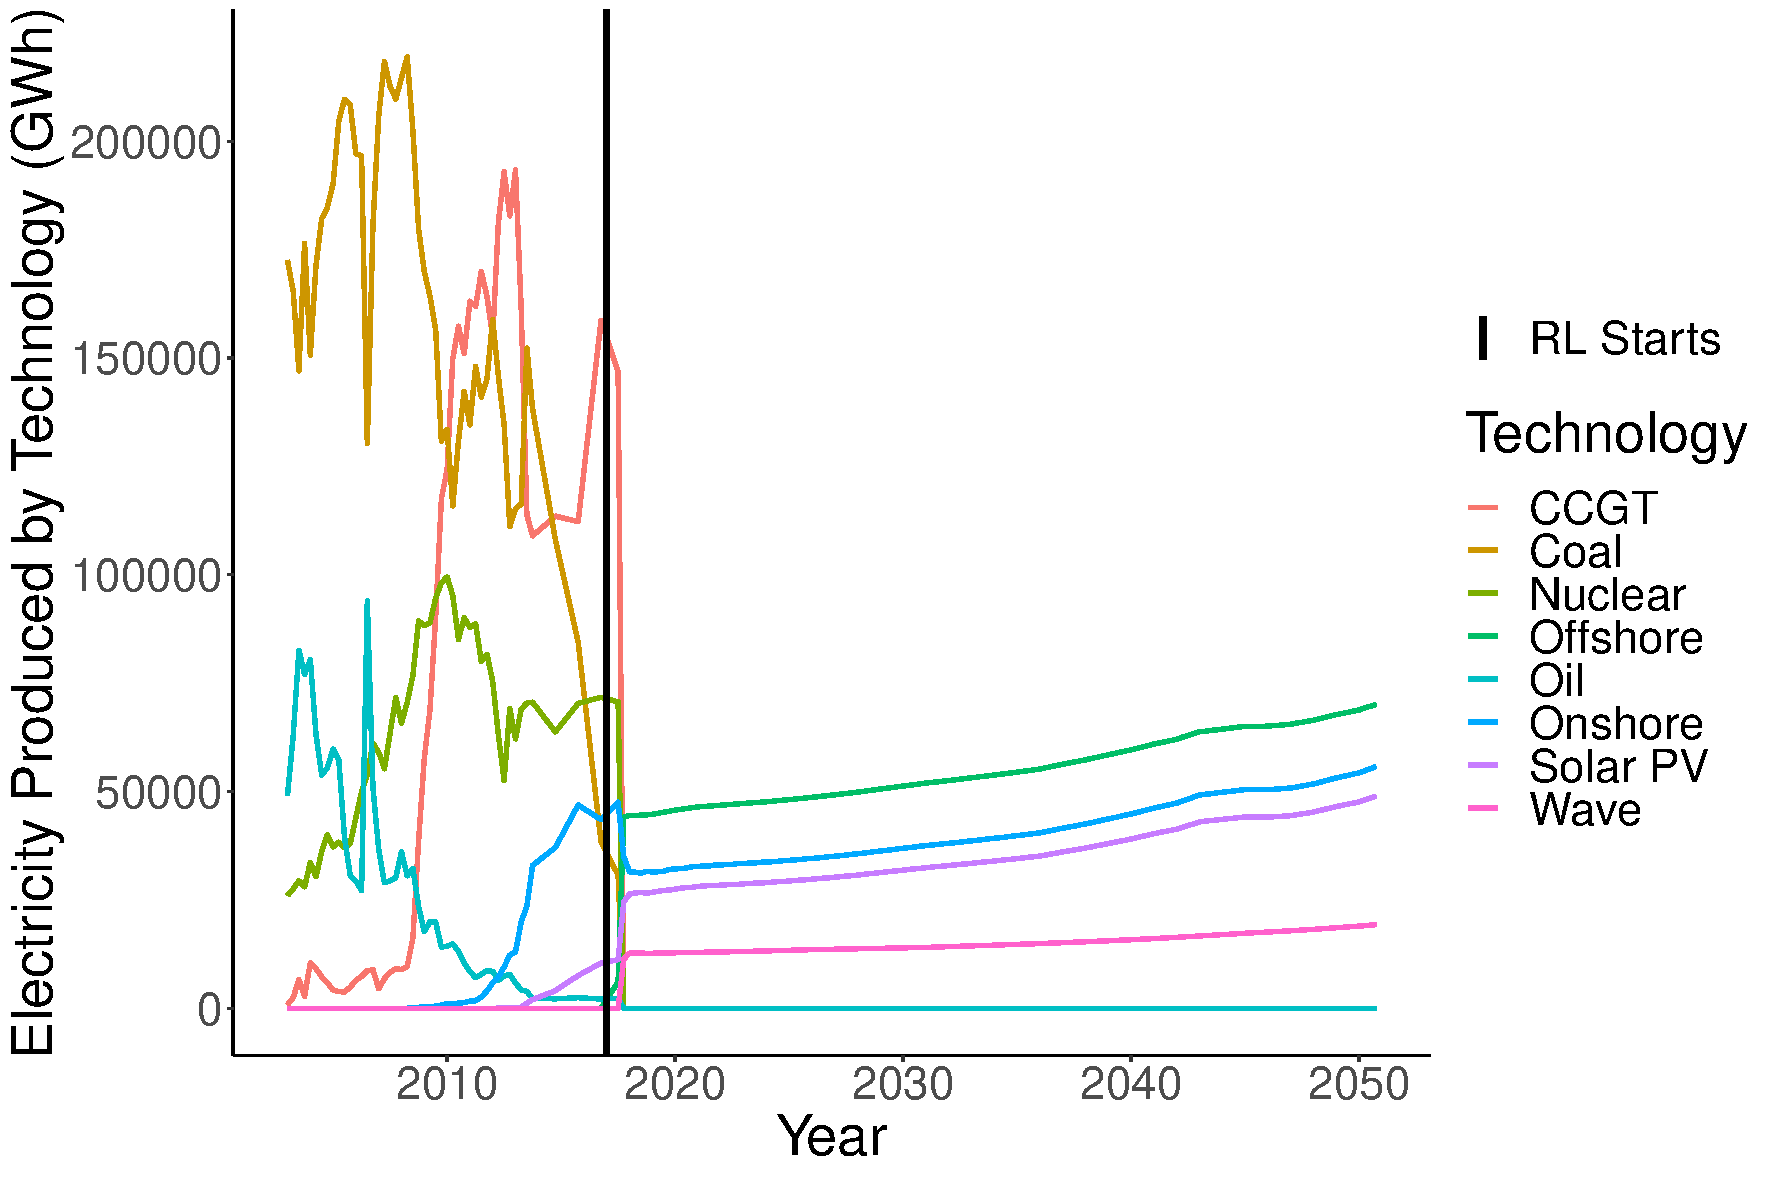
\includegraphics[width=\linewidth]{figures/electricity_generated_plot.pdf}
  \caption{Electricity mix.}
  \label{fig:electricity_generated_plot}
\end{minipage}%
\begin{minipage}{.5\textwidth}
  \centering
  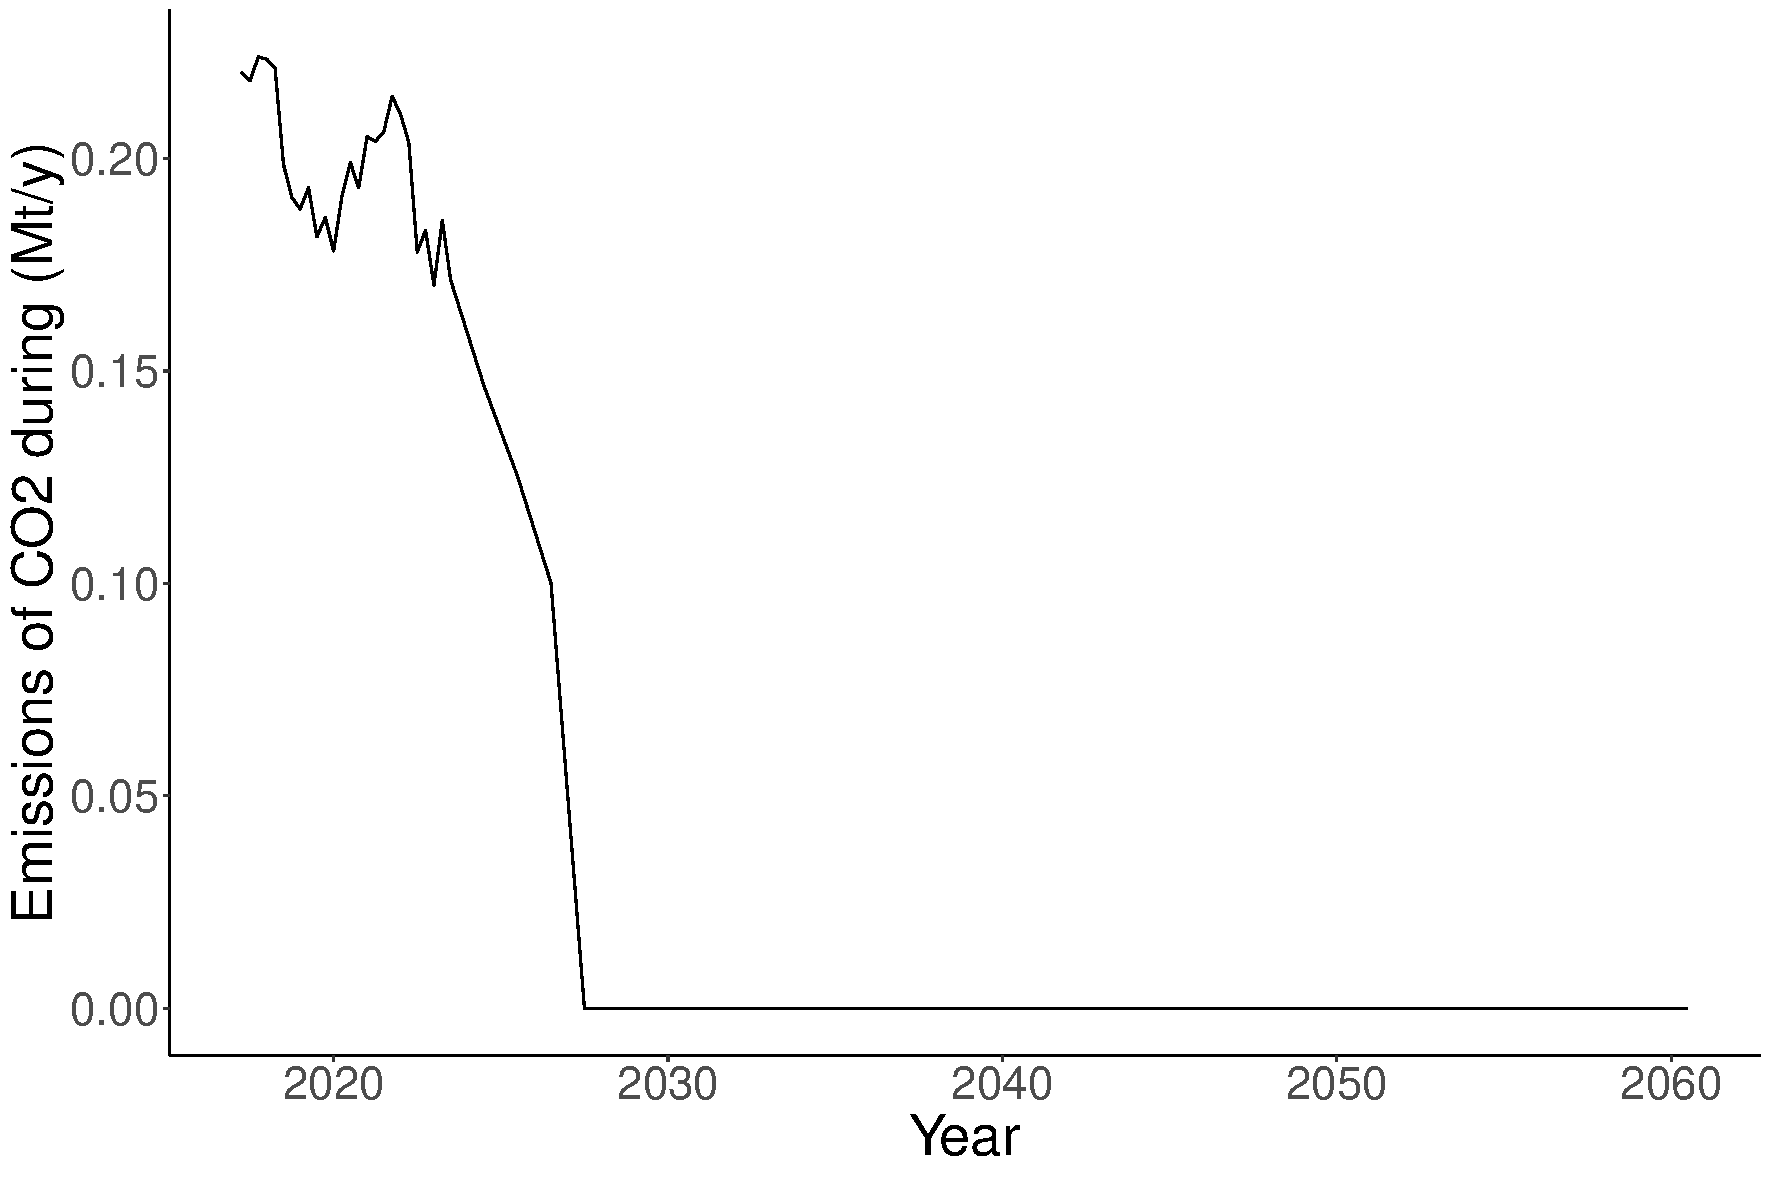
\includegraphics[width=\linewidth]{figures/emissions_plot.pdf}
  \caption{Carbon emissions.}
  \label{fig:emissions_plot}
\end{minipage}
\caption{Simulation metrics over runtime}
\end{figure}



\begin{figure}
\centering
\begin{minipage}{.5\textwidth}
  \centering
  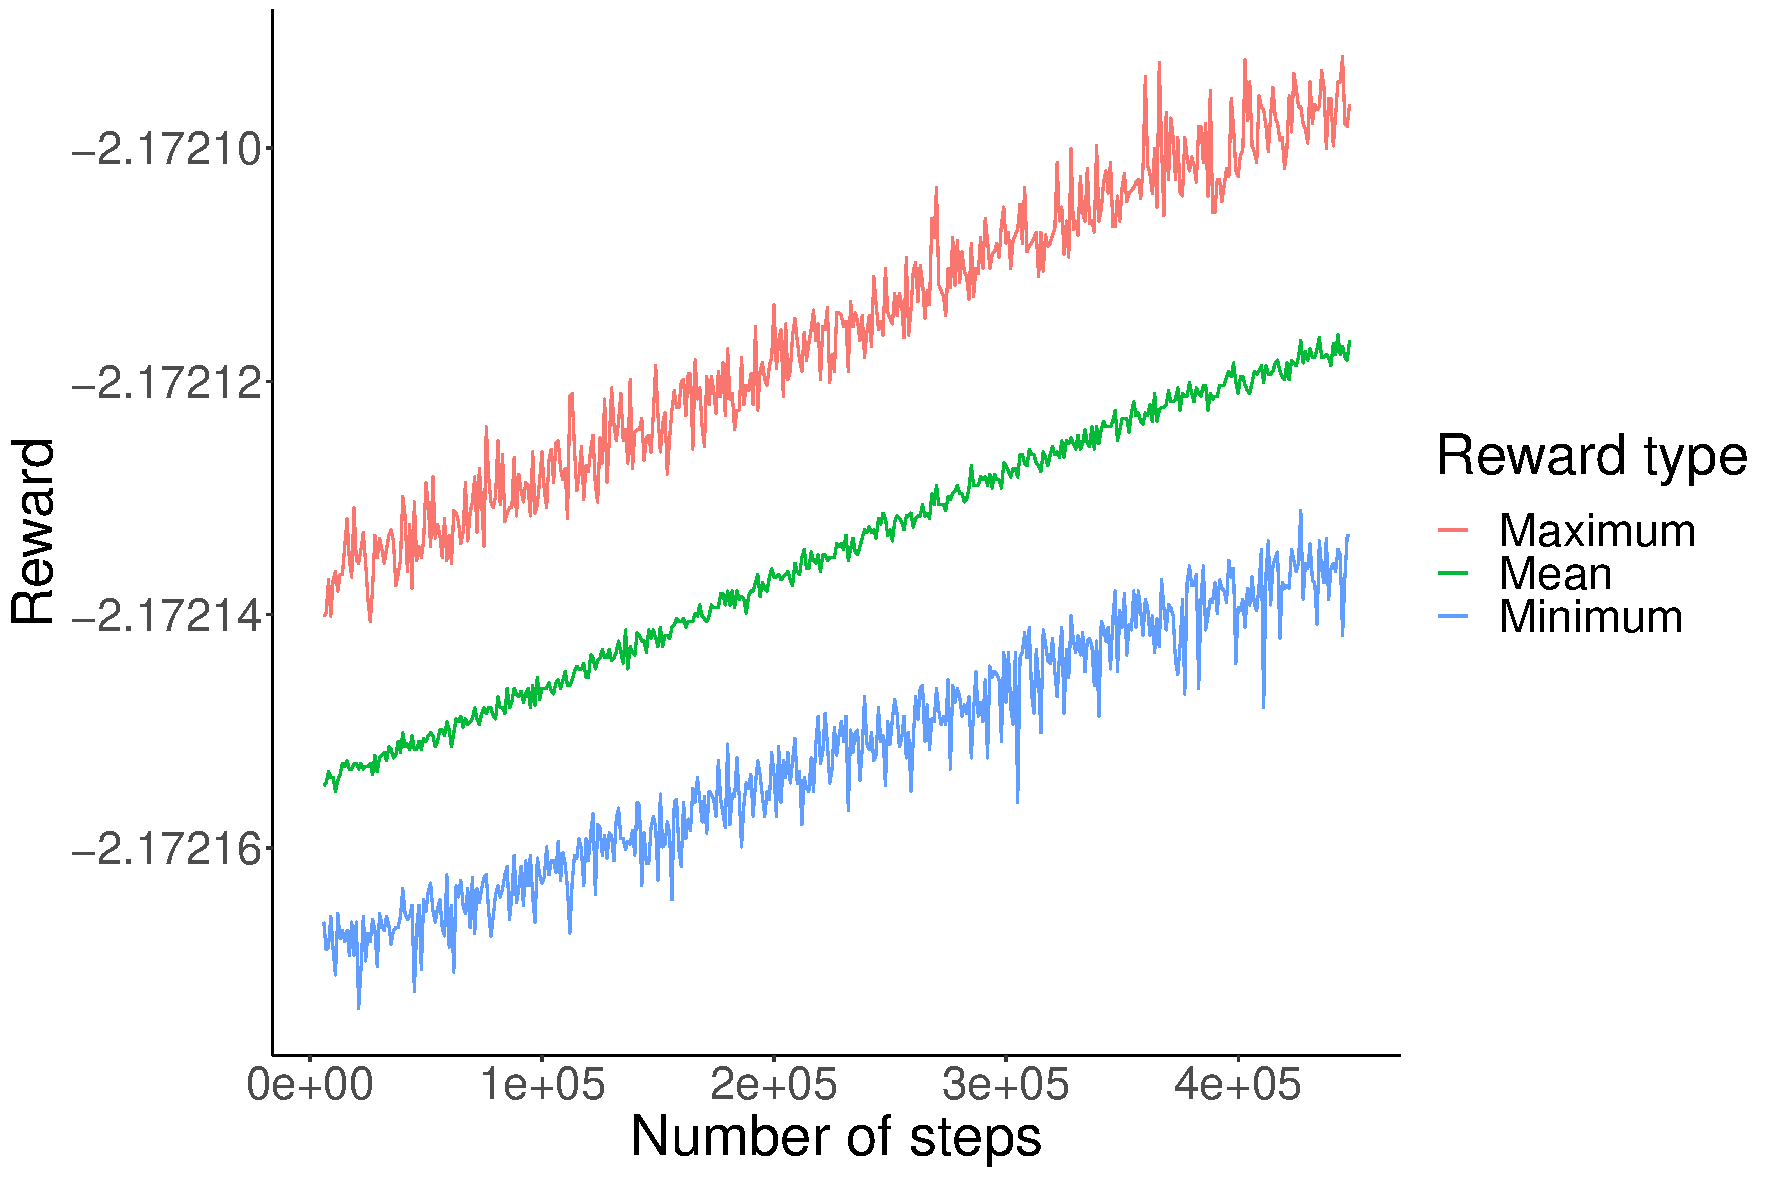
\includegraphics[width=\linewidth]{figures/runtime_steps_plot.pdf}
  \caption{Number of steps.}
  \label{fig:electricity_generated_plot}
\end{minipage}%
\begin{minipage}{.5\textwidth}
  \centering
  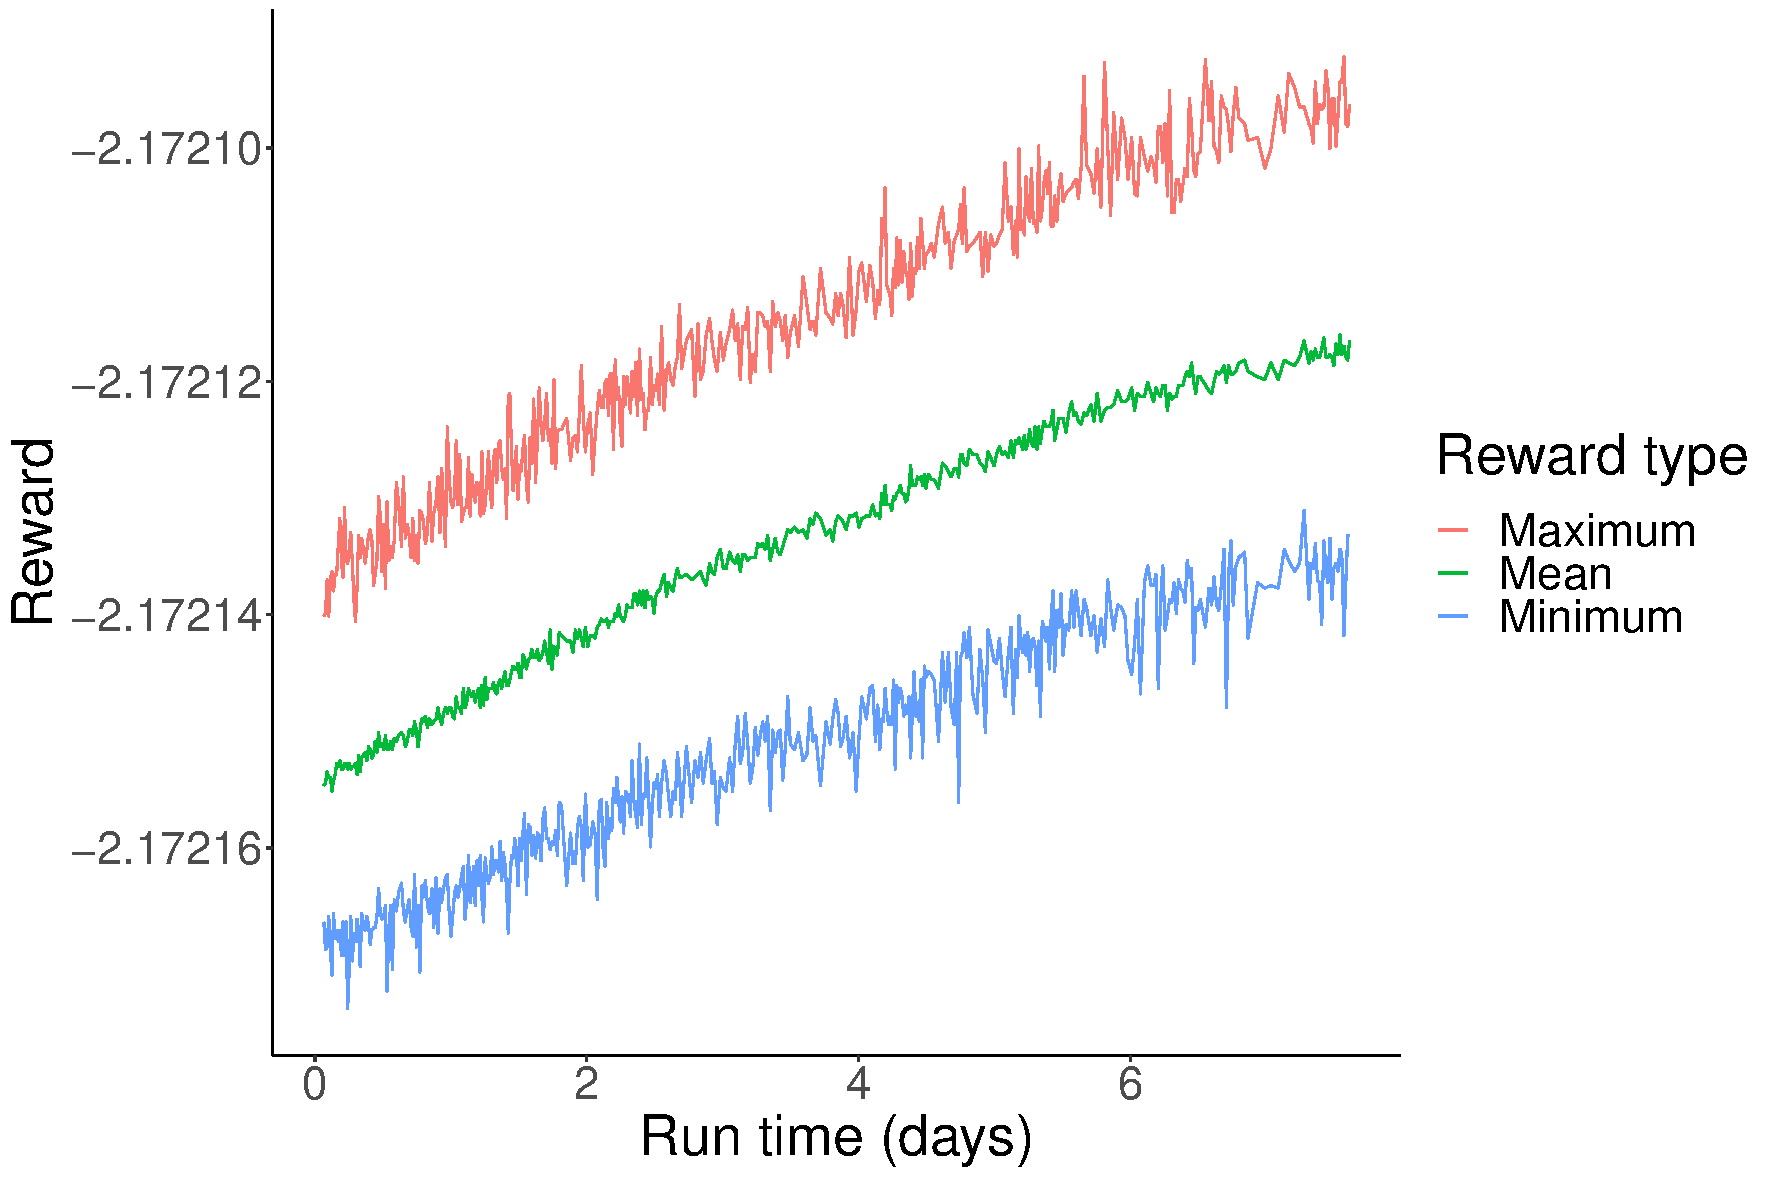
\includegraphics[width=\linewidth]{figures/runtime_days_plot.pdf}
  \caption{Number of days.}
  \label{fig:emissions_plot}
\end{minipage}
\caption{Mean, minimum and maximum rewards over run time.}
\end{figure}





\begin{itemize}
	\item Display electricity mix over time-horizon
	\item Investment in solar, offshore, onshore and wave
	\item Visualise carbon emissions and electricity price over time
	\item Discuss these results and detail 
\end{itemize}


%\section*{References}

\bibliographystyle{ieeetr}
\bibliography{library,ftt-power-custom}

\end{document}
